\documentclass[conference]{IEEEtran}
\IEEEoverridecommandlockouts
% The preceding line is only needed to identify funding in the first footnote. If that is unneeded, please comment it out.
\usepackage{cite}
\usepackage{amsmath,amssymb,amsfonts}
\usepackage{algorithmic}
\usepackage{graphicx}
\usepackage{textcomp}
\usepackage{xcolor}
\def\BibTeX{{\rm B\kern-.05em{\sc i\kern-.025em b}\kern-.08em
    T\kern-.1667em\lower.7ex\hbox{E}\kern-.125emX}}
\begin{document}

\title{Human Mask Generation in Images\\
\thanks{Identify applicable funding agency here. If none, delete this.}
}

\author{\IEEEauthorblockN{Gursimar Singh}
\IEEEauthorblockA{\textit{B.Tech (Final Year), Department of Electronics and Communication Engineering} \\
\textit{PDPM Indian Institute of Information Technology, Design and Manufacturing, Jabalpur}\\
gursimarsingh@iiitdmj.ac.in}
}

\maketitle

\begin{abstract}
Pixel-wise segmentation of objects in natural environments is one of the most discussed problems of modern times in computer vision. Many object detectors gained both popularity and accuracy after state-of-the-art object localization deep learning algorithms were introduced. But a bounding box is not enough for many applications and thus pixel-wise segmentation is required. My work was focused on pixel-wise accurate mask generation of humans in images. I explored and experimented various conventional image processing and modern deep learning models for this task. Human mask generation can be eased if we have information about the pose of the human to be segmented. This not only helps in providing a prior/seed for segmentation but also helps to identify the person in focus in an image. This report summarizes the pros and cons of various approaches. Analysis of each approach has also been done on fixed person dataset from MS-COCO 2017 and PASCAL VOC 2012.\\ 
\end{abstract}
\begin{IEEEkeywords}
Segmentation, Human Pose, Convolution Neural Networks, Conditional Random Fields
\end{IEEEkeywords}

\section{INTRODUCTION}
This document is a model and instructions for \LaTeX.
Please observe the conference page limits. 

\section{LITERATURE REVIEW}

Human mask generation can be modelled as a different problem than that of generic object segmentation. Here, we can take advantage of the essential keypoints of the human body thatrepresent the pose of human body. This pose information tells us about the structure of the human body and thus facilitate segmentation. Previous works where pose information is used for human parsing include the Joint Body-Parsing and Keypoint Estimation Network \cite{jppNet}. This novel joint human parsing and pose estimation network incorporates the multiscale feature connections and iterative location refinement in an end-to-end framework. It detects keypoints as well as generate mask and it has been used as a one of the evaluation baselines in this report. 
 
\subsection{Deep Matching and Deep Flow} \label{DM}

Deep Match is a 6-layer convolution-based algorithm which finds dense correspondences between two images. It was introduced in \cite{deepmatch}. Deep Matching relies on a deep, multi-layer, convolutional architecture designed for matching images. It can handle non-rigid deformations and repetitive textures, can therefore efficiently determine dense correspondences in the presence of significant changes between images.

Deep Flow is an optical flow algorithm based on Deep Match. It computes the flow vectors of each pixel of the query image with respect to the reference image. For the subsequent frames of a video sequences there were about 95\% correspondences detected for each pair.

\subsection{Joint Body Parsing and Keypoint Estimation Network} \label{jpp}
It is a deep convolution neural network which estimates keypoints as well as generate mask for the human body. The mask generated are pixel-wise accurate. The output mask is divided into 20 semantic categories including background. The 19 foreground categories include 6 body parts and 13 clothing categories. From literature study and analysis of the existing approaches the author of JPP Net came up with two conclusions:
\begin{enumerate}
  \item The existing human does not consider human body configuration, meanwhile the information produced by the parsing network can also guide the locations joints
   \item A coarse-to-fine technique used in both parsing and pose networks. In case of parsing networks, it implies using multi-scale features for more precise pixel wise classification.
\end{enumerate} 

The architecture of the network is shown in ``Fig. \ref{fig:JPP_arch}''. The network uses Res-4 and Res-5 from ResNet-101 initially to extract feature maps from input image which are fed to the joint module and parsing module. The results generated are separate and can be obtained individually during inference.
\begin{figure}[htbp]
\centerline{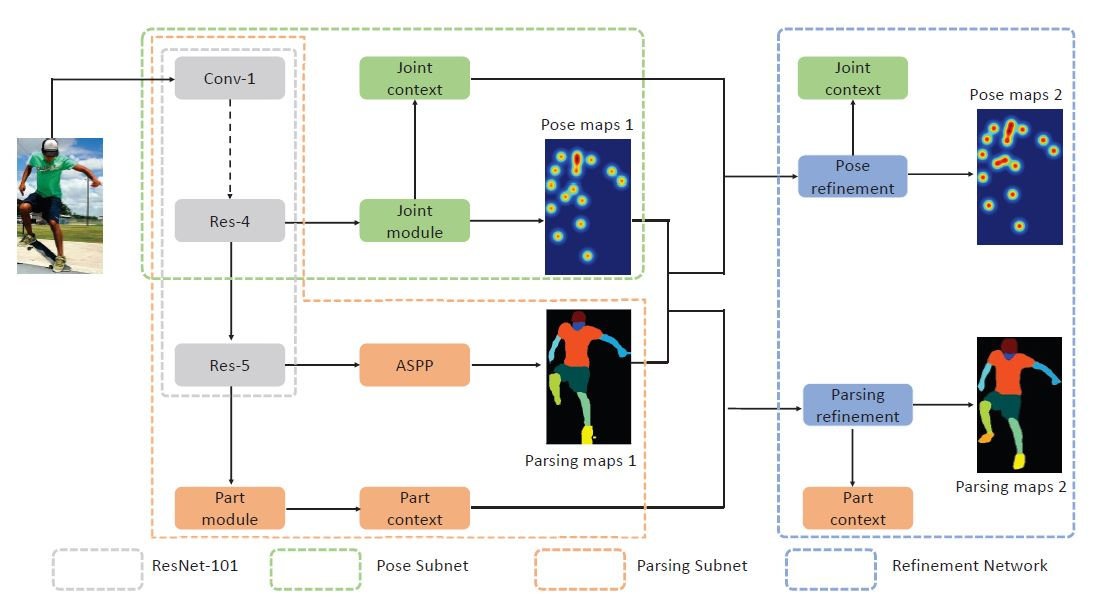
\includegraphics[width=\linewidth]{jpp_net}}
\caption{JPP-Net Architecture}
\label{fig:JPP_arch}
\end{figure}

\subsection{Graph Cut and Cooperative Cut} \label{gc}
Graph cut model the image segmentation problem as an energy minimization problem. There is a sink node and a source node to which all the pixels are connected. The edges are weighted with the probability for each node to belong to the sink/source node. Probabilities are found using the Gaussian foreground and background model which act as edge weights. After this a min cut/max flow algorithm cuts the graph into two parts namely background foreground. A representation of the algorithm is shown in ``Fig. \ref{fig:graph_cut}''. 

Cooperative cut \cite{CoopCut} is an inference method for Markov Random Field (MRF) problem similar to Graph Cut. It introduces a penalizing parameter α for the edges. For image segmentation, this means cooperative cut encourages coherent boundaries, therefore preserving them.
\begin{figure}[htbp]
\centerline{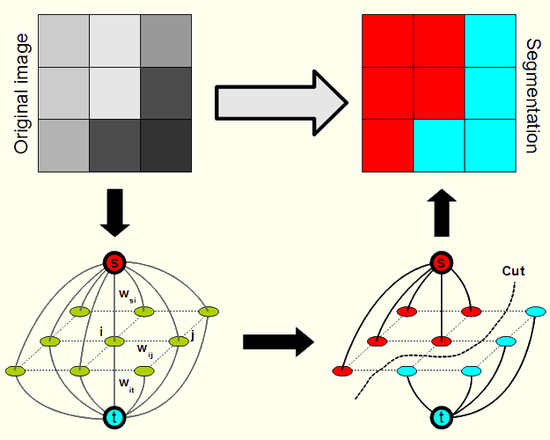
\includegraphics[width=\linewidth]{graph_cut}}
\caption{Graph Cut Segmentation}
\label{fig:graph_cut}
\end{figure}
\subsection{U-Net architecture for image segmentation } \label{un}
U-Net was originally used in \cite{unet} .For biomedical image segmentation. It is an encoder-decoder network with symmetric skip connections. The features from the input image are first extracted using a fully convolutional encoder. The scaled down features are then deconvolved and concatenated in the decoder. After regular interval concatenation of the extracted features and reconstructed features is done using the skip connections. The network arhcitecture is shown in ``Fig. \ref{fig:unet}.'' \\

\begin{figure}[htbp]
\centerline{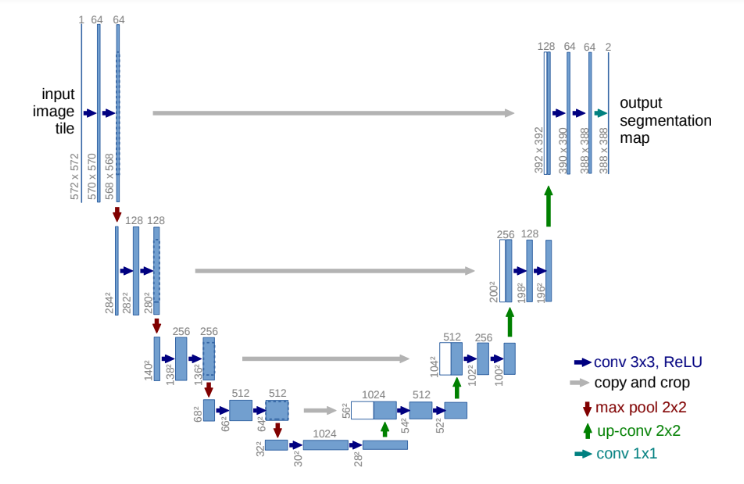
\includegraphics[width=\linewidth]{U-net}}
\caption{U-Net architecture}
\label{fig:unet}
\end{figure}

\section{METHODS}
In order to solve the task of mask generation various methods including conventional algorithms and deep learning approaches were explored. A summary of some of them are mentioned in the following sections. 

\subsection{Keypoint Tracking}
The task of mask generation also involved keypoint tracking in sequence of images for reducing annotation effort in correcting generated keypoints from keypoint detectors like \cite{poseAE}.

The basic approach to track keypoints used was matching features around those keypoints in subsequent frames. Various algorithms like SIFT \cite{sift}, ORB \cite{orb} are available for extracting relevant keypoints and compute their descriptors. But in order to compute descriptors for some specific keypoints open-source implementations of these algorithms cannot be used. Therefore, ORB being open-source algorithm was used by manually providing the keypoints to track and then computing its descriptors. However, this approach did not give good results especially when one or two frames were missing from the sequence. 

Therefore, Deep Match (see section \ref{DM}) was used to find matches between two subsequent frames. As the correspondences found were very dense, the chance that the human keypoints in one frame have corresspondences in other frame was very high. Even if a match for the particluar keypoint was not found, mean of the location of the points lying in its small radius was selected. Kalman Filter was then applied to these predictions in order to facilitate tracking.

\subsection{Identify the Headings}
Headings, or heads, are organizational devices that guide the reader through 
your paper. There are two types: component heads and text heads.

Component heads identify the different components of your paper and are not 
topically subordinate to each other. Examples include Acknowledgments and 
References and, for these, the correct style to use is ``Heading 5''. Use 
``figure caption'' for your Figure captions, and ``table head'' for your 
table title. Run-in heads, such as ``Abstract'', will require you to apply a 
style (in this case, italic) in addition to the style provided by the drop 
down menu to differentiate the head from the text.

Text heads organize the topics on a relational, hierarchical basis. For 
example, the paper title is the primary text head because all subsequent 
material relates and elaborates on this one topic. If there are two or more 
sub-topics, the next level head (uppercase Roman numerals) should be used 
and, conversely, if there are not at least two sub-topics, then no subheads 
should be introduced.

\subsection{Figures and Tables}
\paragraph{Positioning Figures and Tables} Place figures and tables at the top and 
bottom of columns. Avoid placing them in the middle of columns. Large 
figures and tables may span across both columns. Figure captions should be 
below the figures; table heads should appear above the tables. Insert 
figures and tables after they are cited in the text. Use the abbreviation 
``Fig.~\ref{fig}'', even at the beginning of a sentence.

\begin{table}[htbp]
\caption{Table Type Styles}
\begin{center}
\begin{tabular}{|c|c|c|c|}
\hline
\textbf{Table}&\multicolumn{3}{|c|}{\textbf{Table Column Head}} \\
\cline{2-4} 
\textbf{Head} & \textbf{\textit{Table column subhead}}& \textbf{\textit{Subhead}}& \textbf{\textit{Subhead}} \\
\hline
copy& More table copy$^{\mathrm{a}}$& &  \\
\hline
\multicolumn{4}{l}{$^{\mathrm{a}}$Sample of a Table footnote.}
\end{tabular}
\label{tab1}
\end{center}
\end{table}

\begin{figure}[htbp]
\centerline{\includegraphics{fig1.png}}
\caption{Example of a figure caption.}
\label{fig}
\end{figure}

Figure Labels: Use 8 point Times New Roman for Figure labels. Use words 
rather than symbols or abbreviations when writing Figure axis labels to 
avoid confusing the reader. As an example, write the quantity 
``Magnetization'', or ``Magnetization, M'', not just ``M''. If including 
units in the label, present them within parentheses. Do not label axes only 
with units. In the example, write ``Magnetization (A/m)'' or ``Magnetization 
\{A[m(1)]\}'', not just ``A/m''. Do not label axes with a ratio of 
quantities and units. For example, write ``Temperature (K)'', not 
``Temperature/K''.

\section*{Acknowledgment}

The preferred spelling of the word ``acknowledgment'' in America is without 
an ``e'' after the ``g''. Avoid the stilted expression ``one of us (R. B. 
G.) thanks $\ldots$''. Instead, try ``R. B. G. thanks$\ldots$''. Put sponsor 
acknowledgments in the unnumbered footnote on the first page.

\section*{References}

Please number citations consecutively within brackets \cite{b1}. The 
sentence punctuation follows the bracket \cite{b2}. Refer simply to the reference 
number, as in \cite{b3}---do not use ``Ref. \cite{b3}'' or ``reference \cite{b3}'' except at 
the beginning of a sentence: ``Reference \cite{b3} was the first $\ldots$''

Number footnotes separately in superscripts. Place the actual footnote at 
the bottom of the column in which it was cited. Do not put footnotes in the 
abstract or reference list. Use letters for table footnotes.

Unless there are six authors or more give all authors' names; do not use 
``et al.''. Papers that have not been published, even if they have been 
submitted for publication, should be cited as ``unpublished'' \cite{b4}. Papers 
that have been accepted for publication should be cited as ``in press'' \cite{b5}. 
Capitalize only the first word in a paper title, except for proper nouns and 
element symbols.

For papers published in translation journals, please give the English 
citation first, followed by the original foreign-language citation \cite{b6}.

\begin{thebibliography}{00}
\bibitem{b1} G. Eason, B. Noble, and I. N. Sneddon, ``On certain integrals of Lipschitz-Hankel type involving products of Bessel functions,'' Phil. Trans. Roy. Soc. London, vol. A247, pp. 529--551, April 1955.
\bibitem{b2} J. Clerk Maxwell, A Treatise on Electricity and Magnetism, 3rd ed., vol. 2. Oxford: Clarendon, 1892, pp.68--73.
\bibitem{b3} I. S. Jacobs and C. P. Bean, ``Fine particles, thin films and exchange anisotropy,'' in Magnetism, vol. III, G. T. Rado and H. Suhl, Eds. New York: Academic, 1963, pp. 271--350.
\bibitem{b4} K. Elissa, ``Title of paper if known,'' unpublished.
\bibitem{b5} R. Nicole, ``Title of paper with only first word capitalized,'' J. Name Stand. Abbrev., in press.
\bibitem{b6} Y. Yorozu, M. Hirano, K. Oka, and Y. Tagawa, ``Electron spectroscopy studies on magneto-optical media and plastic substrate interface,'' IEEE Transl. J. Magn. Japan, vol. 2, pp. 740--741, August 1987 [Digests 9th Annual Conf. Magnetics Japan, p. 301, 1982].
\bibitem{b7} M. Young, The Technical Writer's Handbook. Mill Valley, CA: University Science, 1989.
\end{thebibliography}
\vspace{12pt}
\color{red}
IEEE conference templates contain guidance text for composing and formatting conference papers. Please ensure that all template text is removed from your conference paper prior to submission to the conference. Failure to remove the template text from your paper may result in your paper not being published.

\end{document}
